\documentclass[11pt]{article}
\usepackage[margin=1in]{geometry}
\usepackage{amsmath,amssymb}
\usepackage{booktabs,enumitem,xcolor,array,tabularx,graphicx,float,longtable}
\usepackage{microtype}
\usepackage{amsthm}
\newtheorem{lemma}{Lemma}
\usepackage[most]{tcolorbox}
\usepackage[colorlinks=true,linkcolor=blue!50!black,citecolor=blue!50!black,urlcolor=blue!50!black]{hyperref}
\newcolumntype{Y}{>{\raggedright\arraybackslash}X}
\newcolumntype{P}[1]{>{\raggedright\arraybackslash}p{#1}}
\setlength{\emergencystretch}{3em}
\setlength{\parskip}{4pt}
\setlength{\parindent}{0pt}
\newcommand{\E}{\mathbb{E}}
\graphicspath{{figures/}}
\hypersetup{pdftitle={RLVR project: the full record}}
\usepackage[capitalize,noabbrev]{cleveref}
\newtcolorbox{idea}[1]{colback=blue!3,colframe=blue!40!black,fonttitle=\bfseries,title=#1,boxrule=0.6pt,arc=2pt}
\newtcolorbox{why}{colback=orange!4,colframe=orange!60!black,fonttitle=\bfseries,title=Why we did it,boxrule=0.6pt,arc=2pt}
\newtcolorbox{found}{colback=green!3,colframe=green!40!black,fonttitle=\bfseries,title=What we found,boxrule=0.6pt,arc=2pt}

\title{\textbf{Same Direction, Different Noise}\\[6pt]
\large The full record of the project: the problem, the literature, every experiment\\ with its reason, design and result, the methods, and where we stand}
\author{Mohamed Ayman\\\small Version 4, October 24, 2026}
\date{}

\begin{document}
\maketitle

\begin{abstract}
\noindent This document records the whole project for a reader who has not followed it: how language models are trained with reinforcement learning on verifiable rewards (RLVR), what the literature claims and where it has gaps, and every experiment we ran, each with its question, reason, pre-registered design, result and consequence. It covers an earlier idea (STOP) and why it was dropped; a theory of the mean and second moment of correctness-only updates; the measurements and tests that led to the main diagnosis (advantage rules trace one accuracy--diversity trajectory and differ in progress rate, with noise as a sufficient cause); the answer-key audit; the first method (coverage-weighted replay, about $+1.2$ points); the 2026 literature and what it changed; base-seeded replay and its controls; the answer-budget check; the matched-accuracy audit of 2026 methods; a pilot of mechanisms that push signal onto rarely solved problems; a transfer probe; a frozen per-problem model of the frontier and its limits; the long Dr.\ GRPO run, which shows that groups of 32 add speed rather than diversity; and the two experiments running now (rollout allocation by frontier value; external versus self-generated information). Appendices give every method's definition and settings and an experiment tracker.
\end{abstract}

\begin{idea}{The idea in one paragraph}RLVR methods that change how sampled answers are scored are usually compared at equal training steps, where a method that progresses more slowly is less sharpened and so has higher pass@$k$. Compared instead at matched pass@1, the advantage rules we tested lie on one accuracy--diversity trajectory on two model families: each rule's expected update on a problem is a multiple of the gradient of its success probability, and the rules differ mainly in noise, which sets the progress rate. Because pass@$k$ at matched pass@1 measures how evenly success is spread across problems, moving the frontier needs signal on rarely solved problems, which a group of 8 rollouts rarely provides. Interventions that add the policy's or the base model's own samples mostly add speed; whether allocating rollouts by frontier value, or adding information the base model lacks, moves the frontier is what the current experiments decide.
\end{idea}

\setcounter{tocdepth}{1}
\tableofcontents
\newpage

%=====================================================================
\section{The problem in plain words}

Large language models can now solve competition math problems. A big part of how they got there is a training method called \textbf{reinforcement learning with verifiable rewards (RLVR)}: the model writes an answer to a math question, a simple program checks whether the final number is right, and the model is nudged to make answers like the right ones more likely and answers like the wrong ones less likely. Repeat this over thousands of questions and the model improves. This recipe is behind DeepSeek-R1 and many open models.

The loop has many design choices that look small but are not:
\begin{itemize}[leftmargin=*,itemsep=1pt]
\item \textbf{How many answers to write per question.} Writing answers is most of the cost of training.
\item \textbf{Which answers to push up or down, and by how much.} For example, reward only the correct answers, or only penalize the wrong ones, or both.
\item \textbf{What to aim for.} Getting one answer right (``pass@1'') or getting at least one right out of several tries (``pass@$k$'', a measure of diversity).
\end{itemize}
Every one of these choices changes three things at once: \emph{which direction} the model is pushed, \emph{how noisy} that push is, and \emph{how much it costs}. Papers usually compare such choices by trial and error, often with unequal compute, one random seed, and small test sets. This project set out to make the effects exact and measurable, and then to test them carefully.

The headline result so far: \textbf{rewarding correct answers and penalizing incorrect answers push the model in the same direction on average; what separates them is noise, and incorrect answers carry most of it.} A well-known paper (Zhu et al., NeurIPS 2025) argued that penalizing incorrect answers is special because it preserves diversity. In our experiments it behaves like a noisier, slower version of rewarding correct answers. Whether that holds for another model family, and whether the noise is truly the \emph{cause}, are the two experiments running now.

%=====================================================================
\section{Background you need}

\begin{idea}{The model as a ``policy''}
A language model given a question $x$ defines a probability $\pi(y\mid x)$ for every possible answer $y$ (a sequence of tokens). Sampling from it at temperature 1 gives a random answer. In RL language the model is a \emph{policy}: it chooses what to say.
\end{idea}

\textbf{Reward.} A verifier compares the answer's final boxed number with the known solution: reward $r=1$ if right, $r=0$ if wrong. For a question, the model's \textbf{success probability} $p$ is the chance that a sampled answer is right.

\textbf{pass@1 and pass@$k$.} pass@1 is the average success probability over test questions (accuracy). pass@$k$ is the fraction of questions where at least one of $k$ sampled answers is right. With $n$ samples of which $c$ are right, the unbiased estimate is $1-\binom{n-c}{k}/\binom{n}{k}$. pass@$k$ at large $k$ measures \emph{coverage} or \emph{diversity}: whether the model can still find the correct answer somewhere among many tries. Training usually raises pass@1 and can lower pass@$k$ at large $k$, because the model becomes confident and repetitive.

\textbf{Policy gradient.} To increase the expected reward, move the model's parameters $\theta$ along its gradient. The classic identity (REINFORCE, Williams 1992) is
\[
\nabla_\theta\,\E[r] = \E\big[r\,\nabla_\theta\log\pi(y\mid x)\big].
\]
The vector $\ell(y)=\nabla\log\pi(y)$ is the answer's \textbf{score}: the direction that makes that answer more likely. So the training update is a sum over sampled answers, $g=\sum_i A_i\,\ell(y_i)$, where $A_i$ is the answer's \textbf{advantage}: positive pushes the answer up, negative pushes it down.

\textbf{Baselines.} Because $\E[\ell(y)]=0$ (probabilities sum to one), subtracting a constant $b$ from every reward, $A=r-b$, does not change the \emph{average} update. It does change its \emph{noise}. This is classical (Williams 1992; Greensmith, Bartlett and Baxter 2004) and matters a lot later.

\textbf{GRPO and Dr.\ GRPO.} The standard recipe samples a \emph{group} of $n$ answers per question (here $n=8$) and uses the group's mean reward as the baseline. GRPO (DeepSeekMath, 2024) also divides by the group's standard deviation and averages each answer's loss over its tokens; Dr.\ GRPO (``GRPO done right'', Liu et al.\ 2025) showed those two divisions bias training and removed them, giving $A_i=r_i-\bar r$. Example: if 2 of 8 answers are right, correct answers get $+0.75$ and wrong ones $-0.25$. Dr.\ GRPO is our main baseline.

\textbf{PSR and NSR.} Two extreme choices studied by Zhu et al.\ (2025): \emph{positive sample reinforcement} (PSR) gives $A=1$ to correct answers and $0$ to wrong ones (only reward successes); \emph{negative sample reinforcement} (NSR) gives $A=-1$ to incorrect answers and $0$ to right ones (only penalize failures). W-REINFORCE, their recommendation, gives $0.1$ to right and $-1$ to wrong.

\textbf{Signal and noise.} Each update is a random vector: its average (over the random answers) is the \emph{signal}, the direction you want; its fluctuation around that average is the \emph{noise}. A noisy update wastes part of each step. In ordinary deep learning, the \emph{gradient noise scale} (McCandlish et al.\ 2018) says how many samples per step are needed before noise stops mattering.

\textbf{Adam.} The optimizer used everywhere. It keeps running averages of each coordinate's gradient (``momentum'') and squared gradient, and divides the first by the square root of the second. A consequence that matters here: more noise in the gradient inflates the denominator, so Adam takes \emph{smaller effective steps} along the signal. Noise therefore slows Adam down.

\textbf{On-policy.} We always sample fresh answers from the current model and update once on them. Many systems (for example the verl framework) reuse each batch of answers for several updates, with a ``clipped'' loss that limits how far the model moves from the one that wrote them.

\textbf{Pre-registration.} Before each experiment we wrote down, in a dated file, the design, the prediction and the rule that decides the verdict, so that results could not quietly reshape the question. All files are in \texttt{experiments/training/PREREGISTRATION\_*.md}.

%=====================================================================
\section{The literature, and where the gaps are}\label{sec:lit}

\subsection{RLVR recipes}
GRPO (Shao et al., DeepSeekMath, 2024) made group-based RL standard for math; DeepSeek-R1 scaled it. Dr.\ GRPO (Liu et al.\ 2025) removed GRPO's length and standard-deviation biases. DAPO (Yu et al.\ 2025) added ``dynamic sampling'': drop questions whose 8 answers are all right or all wrong (they carry no learning signal under a group-mean baseline) and refill the batch.

\subsection{Spending compute on answers: adaptive rollout collection}
Since writing answers dominates cost, many 2025--2026 methods decide adaptively how many answers each question gets: probe a few answers and continue only on questions with mixed results (SPEED-RL, SARA, Pilot-Commit, GRESO), allocate a budget across questions (Knapsack RL, Reinforce-Ada, PAIR), or sample until a correct answer appears. Our review of these papers found recurring evaluation flaws:
\begin{itemize}[leftmargin=*,itemsep=1pt]
\item gains plotted against training \emph{steps} while spending 2 to 3 times more answers per step (for example, SARA's $+6.8$ points comes with 3.3 times the answers);
\item learning rates not retuned, single seeds, 30-problem benchmarks, best checkpoints chosen on the test set;
\item the claimed mechanism (``lower variance'') asserted but never measured.
\end{itemize}

\subsection{Theory of the update}
Davis and Recht (2025) and ARCUS (2026) derive the \emph{average} update of fixed-size groups: on average, a group's update points along $\nabla p$, scaled by a function of $p$. McCandlish et al.\ (2018) introduced the gradient noise scale; Bansal, Mohri, Abreu, Alvarez-Melis and Kakade (``Critical Batch Size for LLM Policy Optimization'', HiLD workshop at ICML 2026) apply it to GRPO, split the noise into a between-question and a within-question part, and find the within-question part dominant. Li et al.\ (2026) study square-root learning-rate scaling; IsoCompute (2026) studies answers per question; Malladi et al.\ (2022) explain square-root scaling for Adam.

\subsection{Assumptions about noise}
Recent variance-reduction papers model the noise with simplifying assumptions. VSR (Wang, Liu and Wang, October 2026) states as Assumption B.3 that the expected squared score norm does not depend on whether the answer was right; BICC (2026) uses a similar approximation. Nobody, to our knowledge, had measured whether right and incorrect answers have different gradient sizes.

\subsection{Does RL add reasoning, or only sharpen it?}
Yue et al.\ (2025) showed that RL-trained models beat their base models at pass@1 but can lose at large $k$: RL may sharpen what the base model already does rather than add new abilities. Wen et al.\ (2025) introduced \textbf{CoT-Pass@$k$}, which counts an answer only if its reasoning is also valid, and argued RL does improve reasoning under that measure. ``Spurious Rewards'' (Shao et al.\ 2025) found that Qwen2.5-Math improves even with random rewards, so small effects on that model family are suspect.

\subsection{Positive versus negative reinforcement}
Zhu et al.\ (``The Surprising Effectiveness of Negative Reinforcement in LLM Reasoning'', NeurIPS 2025) trained with only negative samples (NSR) or only positive samples (PSR). They report that NSR preserves entropy and pass@$k$ while PSR collapses them, credit the negative samples (pushing down incorrect answers redistributes probability to other candidates), and recommend W-REINFORCE. They used 4B to 8B models and $k$ up to 256.

\subsection{Objectives aimed at pass@\texorpdfstring{$k$}{k}}
PKPO (Walder and Karkhanis 2025) and advantage-shaping work (Thrampoulidis et al.\ 2025) give unbiased gradient estimators for pass@$k$, so a model can be trained directly for diversity.

\subsection{The gaps}
\begin{table}[H]
\centering\small
\begin{tabularx}{\linewidth}{@{}P{0.42\linewidth}Y@{}}
\toprule
\textbf{Gap in the literature} & \textbf{What this project does about it}\\
\midrule
The \emph{noise} of adaptive answer-collection rules (random group sizes, early stopping) is not characterized; only the average is. & An exact two-moment theorem: average and noise of any such rule from four numbers per question (Section~\ref{sec:worth}).\\
Nobody measures gradient size separately for right and incorrect answers; recent papers assume they are equal. & We measure it: incorrect answers carry 2.4 to 3.1 times larger squared gradients (Section~\ref{sec:measure}).\\
Adaptive-rollout gains are compared at unequal compute, with one seed. & All our comparisons are at matched generated answers, paired per problem, pre-registered, with at least two seeds.\\
The NSR explanation (negative samples preserve diversity) was never separated from the fact that NSR and PSR differ in noise. & We show their average updates are identical, measure their noise, and compare diversity at \emph{matched accuracy} (Sections~\ref{sec:p4}--\ref{sec:p8}).\\
``Does RL preserve diversity?'' is usually answered at a fixed step, which confuses slower learning with preserved diversity. & We compare runs at equal pass@1: an accuracy-versus-diversity curve.\\
\bottomrule
\end{tabularx}
\end{table}

%=====================================================================
\section{The earlier idea (STOP) and why it failed}

\begin{why}
Before this project, the plan was STOP: a better way to give credit inside an answer. Segment-level RL splits each answer into blocks and credits every block with the change in estimated success across it. STOP asked \emph{where the blocks should end}. Existing methods pick cut points with local scores (token entropy, value variance, EPIG-Tree's gradient-aware score). We showed with exact small examples that a local score can pick the wrong cut, because a cut changes its neighbors and because token gradients interact, and planned a geometry-aware cut rule.
\end{why}

\textbf{The theory worked.} The update error splits exactly into a part that ignores gradient geometry and an interaction part; the interaction vanishes when token gradients are orthogonal; a cut's benefit depends on the other cuts only through its two neighbors.

\begin{found}
In Qwen2.5-Math-1.5B, gradients at different positions are almost orthogonal (median $|\cos|\le0.005$) and the small interactions cancel in aggregate (about $\pm1\%$). In a pre-registered test over all partitions of a 64-token grid, interactions reversed only 2.2\% of orderings, none statistically clear, and never changed the best single cut; the geometry-free score lost at most 1.3\% of the available gain. The effect STOP was built to exploit is real in constructed examples but too small in a real model to matter. Written up honestly as ``local scores suffice'' (TMLR or workshop level).
\end{found}

\textbf{What we kept:} exact per-answer gradient measurement tools, and the habit of \emph{measuring the mechanism before building a method}. Both made the next project possible.

%=====================================================================
\section{What is each generated answer worth? (WORTH)}\label{sec:worth}

\begin{why}
Generating answers is the main cost of RLVR, and the adaptive-collection literature (Section~\ref{sec:lit}) compares rules by heuristics. If the value of each answer could be computed exactly, rules could be ranked, and the best rule derived instead of guessed.
\end{why}

\subsection{The two-moment theorem}
Let $p$ be a question's success probability, $F_1$ and $F_0$ the average squared score size $\E\|\ell\|^2$ of right and of incorrect answers, and $\|\nabla p\|^2$ the size of the question's learning signal. Two simple facts drive everything: a correct answer's average score is $\nabla p/p$ and a incorrect answer's is $-\nabla p/(1-p)$; and given its reward, an answer is independent of the others.

\begin{idea}{Theorem (two moments of any reward-adapted rule)}
For any rule that decides when to stop sampling and which advantages to give using only the rewards seen so far (including random group sizes, early abandonment, sampling until success, and filtering),
\[
\E g = c(p)\,\nabla p,\qquad \E\|g\|^2 = F_1 D_1(p) + F_0 D_0(p) + \|\nabla p\|^2 X(p),
\]
where $c, D_1, D_0, X$ and the expected cost depend only on the rule and on $p$. So the average, the noise and the cost of the update depend on a question only through \textbf{four numbers}: $p$, $\|\nabla p\|^2$, $F_0$, $F_1$.
\end{idea}

\textbf{Why it is true, in one line:} condition on the whole sequence of rewards; then the stopping time and the advantages are fixed numbers and the answers are independent, so averaging over answers and then over rewards gives both formulas. No optional-stopping argument is needed. \textbf{What is new} is the noise part with separate $F_0$, $F_1$ and random group sizes; the average part for fixed groups was known (Davis and Recht; ARCUS). All statements are verified by exact enumeration in small models (\texttt{theory/exact.py}).

\subsection{Consequences: ranking the rules and the optimal rule}
Treating questions as having unrelated gradients and choosing the step size optimally, the progress per generated answer is proportional to $\text{signal}^2/(\text{cost}\times\text{second moment})$. Dynamic programming over the counts of (wrong, right) answers seen so far gives the \textbf{optimal rule}: after each block of 4 answers, a lookup table says stop or continue, and which advantages to give.

\begin{table}[H]
\centering\small
\begin{tabularx}{\linewidth}{@{}P{0.42\linewidth}YYYY@{}}
\toprule
\textbf{Rule (efficiency relative to the optimal rule)} & \textbf{Uniform} & \textbf{Mostly hard} & \textbf{U-shaped} & \textbf{Mostly easy}\\
\midrule
Fixed group of 8 (GRPO, Dr.\ GRPO, DAPO) & 0.61 & 0.38 & 0.40 & 0.38\\
Fixed group of 16 & 0.65 & 0.41 & 0.43 & 0.41\\
Probe 4, abandon if all agree, fill to 16 & 0.77 & 0.60 & 0.67 & 0.60\\
Sample until 1 correct, cap 16 & 0.26 & 0.09 & 0.12 & 0.30\\
\bottomrule
\end{tabularx}
\caption{Exact efficiency by difficulty mix. DAPO's filtering has exactly the efficiency of the group it filters; sample-until-correct is worst; probe-then-fill is the best rule in use.}
\end{table}

\subsection{When does a better rule matter? The critical budget}
Without assuming unrelated question gradients, one step's progress at $B$ answers per step is $\langle\nabla J,\mu\rangle^2/(2L(s+nV/B))$, with $s$ the squared size of the mean update and $V$ its noise. The \textbf{critical budget} $B^\star=nV/s$ splits two regimes: below it, a rule $k$ times more efficient is worth $k$ times the answers (about $\sqrt k$ under Adam at a fixed learning rate); above it, no reweighting helps (Figure~\ref{fig:regime}). This later turned out to be already published for GRPO (Bansal et al.), so it became background.

\begin{figure}[H]
\centering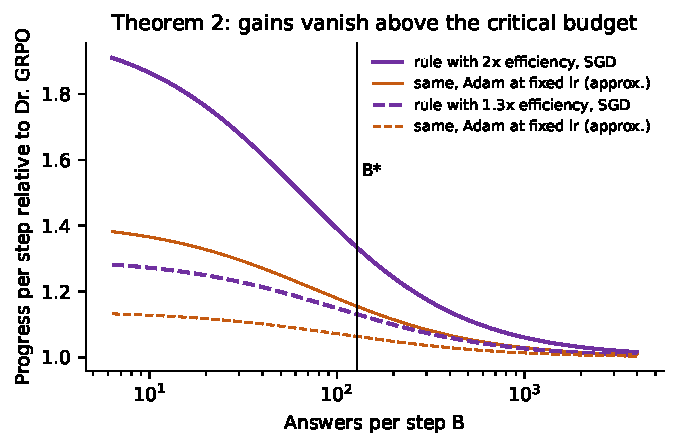
\includegraphics[width=0.5\linewidth]{regime.pdf}
\caption{Predicted gain of a better rule against answers per step: gains vanish above the critical budget, and Adam turns a gain of $k$ into about $\sqrt k$.}
\label{fig:regime}
\end{figure}

%=====================================================================
\section{Measuring the four numbers}\label{sec:measure}

\begin{why}
The theory's predictions depend on two unknowns: how $F_0$ compares with $F_1$, and how the learning signal $\|\nabla p\|^2$ varies with difficulty. Both had to be measured in a real model before any prediction meant anything.
\end{why}

\begin{found}
\textbf{Incorrect answers carry larger gradients.} In Qwen2.5-Math-1.5B (exact per-answer gradients on MATH training problems): in the last-layer block, 40 questions by 16 answers, $F_1/F_0=0.36$ (90\% intervals do not overlap), while incorrect answers are only 9\% longer (421 against 386 tokens). Over all 1.5B parameters, measured before every training run: $F_1/F_0$ between 0.32 and 0.42, so \textbf{incorrect answers carry 2.4 to 3.1 times larger squared gradients}. Likely reason: incorrect answers contain more low-probability tokens, whose scores are large. This contradicts VSR's Assumption B.3.

\textbf{The learning signal fades at both ends.} With 96 answers per question, the estimated $\|\nabla p\|^2$ is $0.73\pm0.60$ on very easy or very hard questions and $15.5\pm5.4$ on medium ones; the best fit is $p^2(1-p)^2$, and a flat shape is rejected (Figure~\ref{fig:shape}). This makes the optimal rule robust: it should spend answers on medium questions.
\end{found}

\begin{figure}[H]
\centering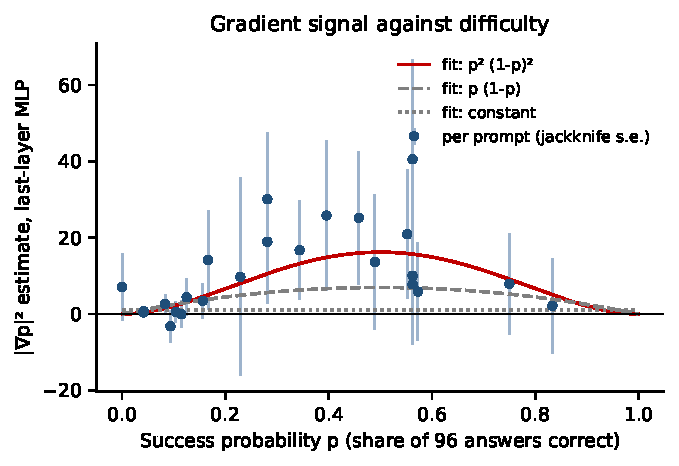
\includegraphics[width=0.5\linewidth]{shape.pdf}
\caption{Per-question learning signal against success probability, with three candidate shapes.}
\label{fig:shape}
\end{figure}

%=====================================================================
\section{First tests of the theory}

\subsection{Pre-registration 1: scale down incorrect answers (pilot)}
\begin{why}
The simplest consequence of $F_0>F_1$: weight each incorrect answer's advantage by $w=F_1/F_0$. A one-line change to Dr.\ GRPO, predicted to raise efficiency by 1.1 to 1.6 times in 11 of 12 settings.
\end{why}
\textbf{Design.} Qwen2.5-Math-1.5B base, 3,920 numeric MATH training problems (four subjects), 16 questions by 8 answers per step, 150 steps, 512-token answers, AdamW at $10^{-6}$; Dr.\ GRPO against the scaled version; two seeds; primary: greedy accuracy on the 364 numeric MATH-500 problems. \textbf{Prediction:} promising if at least $+2$ points in both seeds.
\begin{found}
No gain: 45.3\% against 47.5\% (seed 1), 44.0\% against 46.7\% (seed 2). Verdict: \textbf{no evidence}. Lesson: under Adam at a fixed learning rate, a 1.1 to 1.6 times efficiency gain shrinks to 1.06 to 1.25 times, too small to see with two seeds.
\end{found}

\begin{figure}[H]
\centering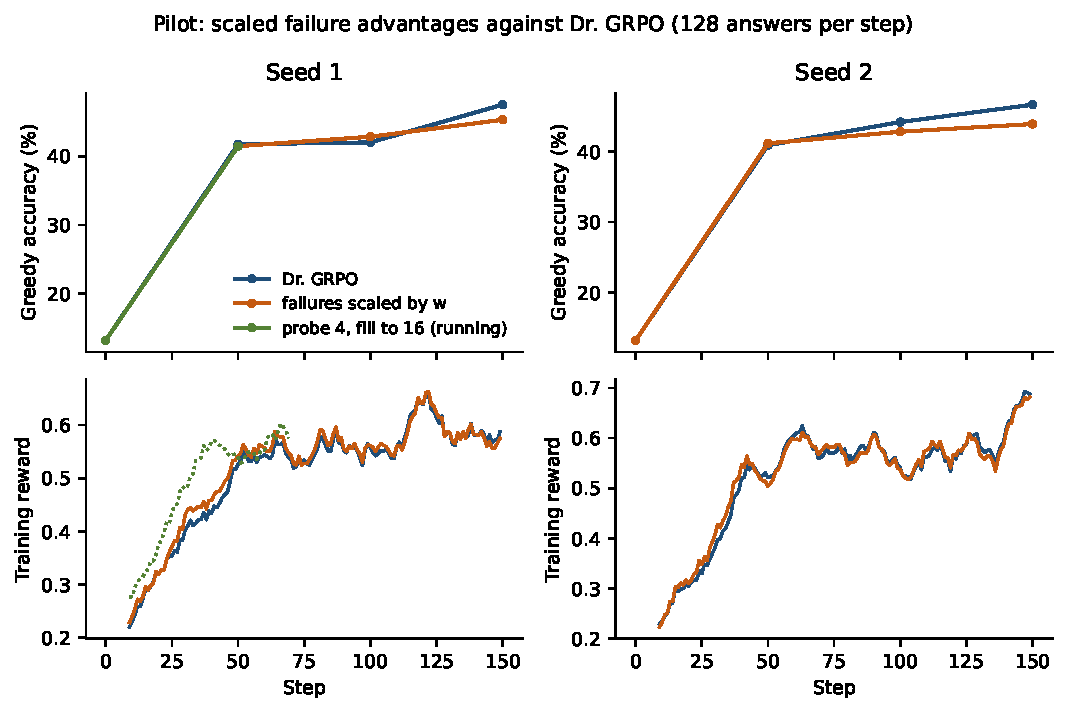
\includegraphics[width=0.8\linewidth]{pilot.pdf}
\caption{Pilot: scaled failures (orange) track Dr.\ GRPO (blue).}
\end{figure}

\subsection{Pre-registrations 2 and 3: collection rules at equal cost, and measuring noise inside training}
\begin{why}
The optimal rule predicts a larger gain (1.7 to 2.3 times Dr.\ GRPO's efficiency). Testing it fairly needs exactly matched generated answers. And to know \emph{why} a rule helps or not, we needed to measure signal and noise during training, not just accuracy.
\end{why}
\textbf{Design.} The optimal rule (lookup table re-solved every 10 steps from the recent difficulty mix), probe-then-fill, scaled failures, and Dr.\ GRPO at several budgets (32 to 256 answers per step), all at matched answers (19,200 over 150 steps for the 128-answer arms), two seeds, paired per problem on 3,382 held-out MATH test problems. \textbf{New tool:} at every step the questions are split at random into two halves; inner products of the two halves' gradients, and of each half with an independent unbiased reference for the population gradient, give the signal, the noise and the noise scale, without extra sampling. \textbf{Prediction:} promising if the optimal rule beats Dr.\ GRPO by at least 1.5 points in both seeds.
\begin{found}
\begin{itemize}[leftmargin=*,itemsep=1pt]
\item Optimal rule: $+1.1\pm0.4$ (seed 1) and $+3.3\pm0.5$ (seed 2) points, with matched answers (19,172 and 19,200) and about 1\% more tokens. Positive in both seeds, but the pre-registered bar (1.5 in both) was \textbf{missed} because of seed 1.
\item Probe-then-fill: $+2.0$ and $+0.8$ (MATH-500). Scaled failures: $-0.4$ and $+1.1$. Fewer answers clearly hurts: 32 against 128 answers per step, $-4.4$ points (seed 1; not every rung of the budget ladder obtained GPUs).
\item Training becomes noise-limited as it plateaus: Dr.\ GRPO's noise scale grows from about 900 answers (steps 0 to 49) to over 10,000 (steps 50 to 149): the shared signal shrinks while the noise does not.
\item Gains are much smaller than one-step theory predicts, consistent with Adam's square-root effect.
\end{itemize}
\end{found}

%=====================================================================
\section{The literature check and the change of direction}

\begin{why}
Before investing more, we checked carefully (three literature reviews, key claims verified by hand) whether the framing was new.
\end{why}
\begin{found}
\begin{itemize}[leftmargin=*,itemsep=1pt]
\item \textbf{The critical-budget framing was taken} (Bansal et al., HiLD at ICML 2026), including the finding that within-question noise dominates.
\item The common evaluation flaws listed in Section~\ref{sec:lit}.
\item \textbf{No paper measures gradient norms by correctness}, as far as we found, and none separates the average and the noise of positive and negative reinforcement.
\end{itemize}
\end{found}
So the main question moved to positive versus negative reinforcement, where our theorem and our measurement give something nobody else has. The optimal-rule result stays as a practical side result.

\subsection{The key observation}
Give each correct answer advantage $a$ and each incorrect answer $b$. The theorem gives
\[
\E g = n(a-b)\,\nabla p,\qquad \text{noise}\approx n\big(a^2pF_1+b^2(1-p)F_0\big).
\]
\begin{itemize}[leftmargin=*,itemsep=1pt]
\item PSR ($a=1,b=0$) and NSR ($a=0,b=-1$) both have average $n\nabla p$: \textbf{exactly the same expected update}. (This is the classical baseline invariance; the new part is the noise and its measurement.)
\item In fact NSR $=$ PSR $-\sum_i\nabla\log\pi(y_i)$, and the extra term has average exactly zero: it is pure noise.
\item PSR's noise $npF_1$ sits on easy questions; NSR's $n(1-p)F_0$ on hard ones. With $F_0\approx2.5F_1$, NSR is noisier on every question solved less than 71\% of the time.
\item The whole family $A=r-b$ shares the average; its noise is smallest near $b^\star=pF_1/(pF_1+(1-p)F_0)\approx0.15$.
\end{itemize}
\textbf{Consequence:} to first order, any difference between PSR and NSR (entropy, pass@$k$) must come from the noise, from an optimizer that reacts to noise (Adam), or from implementation choices outside the theorem.

%=====================================================================
\section{PSR against NSR (Pre-registration 4)}\label{sec:p4}

\begin{why}
Test the observation directly: if NSR's famous diversity advantage is real in clean on-policy training with equal averages, it must be a noise effect; if it does not appear, it must come from implementation.
\end{why}
\textbf{Design.} Dr.\ GRPO, PSR, NSR, W-REINFORCE; two seeds; strictly on-policy; in-training noise measurement; an on-policy entropy probe (the first four answers of every question, identical for all rules); pass@$k$ with 64 samples at step 150. \textbf{Prediction:} separation if NSR beats PSR by at least 3 points of pass@64, or has at least 20\% more entropy, in both seeds.

\begin{table}[H]
\centering\small
\resizebox{\linewidth}{!}{\begin{tabular}{@{}lcccc@{}}
\toprule
\textbf{Rule} (seed 1 / seed 2) & \textbf{Training acc., steps 25--49} & \textbf{pass@1 at 150} & \textbf{pass@64 at 150} & \textbf{Entropy, 100--150}\\
\midrule
Dr.\ GRPO & 50.6 / 48.0 & 43.3 / 43.2 & 83.2 / 81.9 & 0.227 / 0.224\\
PSR (reward right only) & 51.3 / 48.2 & 42.4 / 42.0 & 83.2 / 83.8 & 0.227 / 0.226\\
NSR (penalize wrong only) & 33.6 / 36.4 & 37.7 / 39.1 & 83.0 / 82.1 & 0.251 / 0.251\\
W-REINFORCE & 38.6 / 38.0 & 38.5 / 39.8 & 80.5 / 81.3 & 0.243 / 0.256\\
\bottomrule
\end{tabular}}
\caption{Untrained model: pass@1 13.8, pass@64 79.9.}
\end{table}

\begin{found}
NSR's measured noise is 6.4 times PSR's (theory about 7). NSR learns clearly more slowly, ends with lower pass@1, and reaches the \emph{same} pass@64; its entropy is only 11\% higher. The measured noise matches the theorem within 30\% for every rule. Verdict: \textbf{the separation is not reproduced} in either seed. W-REINFORCE, the NSR paper's recommendation, has the lowest pass@64.
\end{found}

\begin{figure}[H]
\centering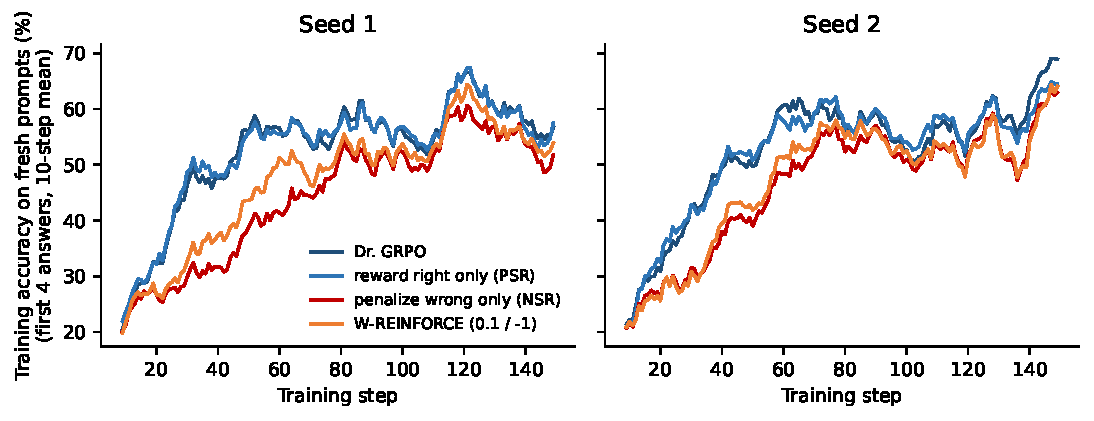
\includegraphics[width=0.85\linewidth]{pn_curves.pdf}
\caption{Training accuracy on fresh questions. The noisy rules, dominated by incorrect answers, learn about twice as slowly.}
\end{figure}

\begin{figure}[H]
\centering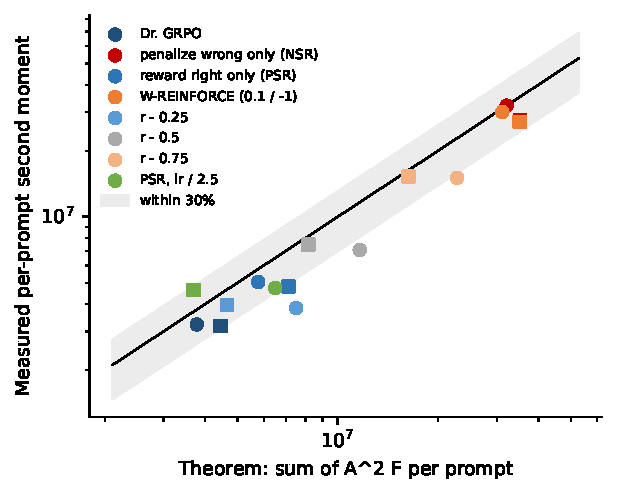
\includegraphics[width=0.45\linewidth]{noise_validation.pdf}
\caption{Measured gradient noise against the theorem's prediction from $F_0$, $F_1$ and the observed reward counts; shaded: within 30\%.}
\end{figure}

%=====================================================================
\section{Matched accuracy, and the NSR paper's own implementation}

\subsection{Pre-registration 5: is NSR just a slower PSR?}
\begin{why}
At a fixed step, a slower run looks more diverse simply because it has learned less. The fair comparison is diversity \emph{at the same accuracy}: for each NSR checkpoint, interpolate PSR's pass@32 at the same pass@1 along PSR's trajectory and take the difference. This gives an \textbf{accuracy-versus-diversity curve} per run.
\end{why}
\textbf{Design.} PSR and NSR, seeds 3 and 4, pass@32 from 32 samples on 128 MATH-500 problems at steps 0 to 150. \textbf{Prediction:} the matched difference is below 2 points in both seeds.
\begin{found}
NSR is 2.1 points \emph{below} PSR's curve (seed 3) and 0.2 below (seed 4). \textbf{No extra diversity at equal accuracy} (Figure~\ref{fig:frontier}, left).
\end{found}

\subsection{Pre-registration 6: do the NSR paper's implementation choices create the effect?}
\begin{why}
Zhu et al.\ used verl, which differs from clean training in three ways the theorem does not cover: each batch of answers is reused for 4 updates with clipping (stale samples), each answer's loss is averaged over its tokens, and PSR and NSR average over only the answers they train on. If the effect lives anywhere, it may live there.
\end{why}
\textbf{Design.} All three choices reproduced at matched answers and updates (with fresh samples, our clipped loss equals the plain loss exactly). \textbf{Prediction:} recreated if NSR beats PSR by 3 points of pass@32, or 20\% entropy, in both seeds.
\begin{found}
NSR learns even more slowly here (training accuracy 31.0 and 31.4 against 43.0 and 45.4), and at step 150 its pass@32 is 7.0 and 1.6 points \emph{lower} than PSR's; its entropy is 1.11 and 1.18 times PSR's; at matched pass@1 the differences are $+0.3$ and $-1.3$. Verdict: \textbf{not recreated}. Disclosure found later: per-token averaging makes gradients larger, so the gradient clipping at norm 1 (verl's default) was active on 26 to 28\% of NSR's steps and 7 to 8\% of PSR's; it never triggered in any other on-policy run.
\end{found}

\begin{figure}[H]
\centering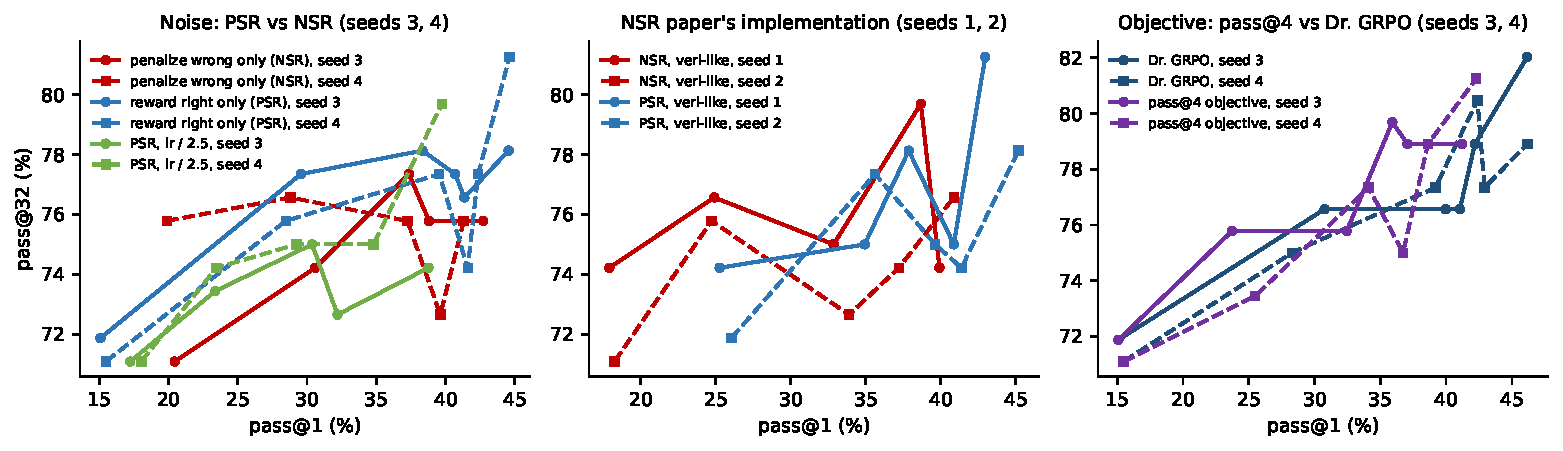
\includegraphics[width=0.95\linewidth]{frontier.pdf}
\caption{Accuracy (pass@1) against diversity (pass@32) during training, 128 problems. Left: changing the noise (PSR, NSR, PSR at a lower learning rate). Middle: the NSR paper's implementation. Right: changing the objective (pass@4 against Dr.\ GRPO). No run separates from its reference beyond the evaluation noise (point comparisons, not yet an equivalence test).}
\label{fig:frontier}
\end{figure}

%=====================================================================
\section{Same average, graded noise (Pre-registration 7)}

\begin{why}
The strongest test of ``only noise differs'' available with one family: the baselines $A=r-b$ for $b=0, 0.25, 0.5, 0.75, 1$ all have exactly the same average update, but the theory predicts different noise. If learning speed follows the predicted noise, noise is the likely cause. A PSR run with the learning rate divided by 2.5 tests the ``slower clock'' reading: does NSR look like PSR run more slowly?
\end{why}

\begin{table}[H]
\centering\small
\resizebox{\linewidth}{!}{\begin{tabular}{@{}lcccccc@{}}
\toprule
& $b=0.25$ & $b=0$ (PSR) & $b=0.5$ & $b=0.75$ & $b=1$ (NSR) & PSR, lr $/2.5$\\
\midrule
Predicted noise vs PSR & 0.81$\times$ & 1$\times$ & 1.25$\times$ & 2.5$\times$ & about 6$\times$ & 1$\times$\\
Steps to 45\% training accuracy, seed 3 & 37 & 44 & 44 & 53 & 56 & 84\\
Steps to 45\% training accuracy, seed 4 & 38 & 33 & 41 & 45 & 56 & 76\\
pass@32 vs PSR at equal pass@1, seed 3 & $+0.0$ & 0 & $+0.8$ & $-0.8$ & $-2.1$ & \\
pass@32 vs PSR at equal pass@1, seed 4 & $+0.2$ & 0 & $+2.1$ & $+0.6$ & $-0.2$ & \\
\bottomrule
\end{tabular}}
\end{table}

\begin{found}
\begin{itemize}[leftmargin=*,itemsep=1pt]
\item \textbf{Speed follows predicted noise} in both seeds (rank correlation 0.9 to 0.97; pre-registered threshold 0.8): passed.
\item The noise formula is within 30\% in all seed-4 runs but only 0.51 to 0.73 in seed 3, so 12 of 16 runs overall; likely because gradient sizes are measured once, before training, and shrink as the model sharpens.
\item Every run stays within about $\pm2$ points of PSR's curve; ``noise adds exploration'' is rejected. The strict slower-clock rule asked for every difference below 2 and two were 2.07 and 2.14: \textbf{formally inconclusive}. PSR at a 2.5 times lower learning rate learns \emph{more} slowly than NSR, so NSR equals a smaller slowdown.
\end{itemize}
\end{found}

%=====================================================================
\section{Changing the objective, and grading the reasoning (Pre-registration 8)}\label{sec:p8}

\begin{why}
If noise only changes speed, perhaps changing \emph{what the update aims at} moves the curve. We aimed the update exactly at pass@4: per-answer weights from the unbiased pass@$k$ estimator with a leave-one-out baseline, verified over all 256 reward patterns to average $2\cdot4(1-p)^3\nabla p$, the pass@4 gradient (such objectives are known, e.g.\ PKPO; here it is a control). It pushes hard questions and leaves solved ones alone. We also graded the reasoning, not just the final number, because a diversity gain could hide lucky guesses.
\end{why}
\textbf{Prediction:} the curve moves if pass@4 training is at least 2 points of pass@32 above Dr.\ GRPO at equal pass@1 in both seeds.
\begin{found}
$+1.6$ (seed 3) and $+0.2$ (seed 4): \textbf{curve fixed}. At step 150 pass@4 training simply has lower pass@1 (41 to 42 against 46). With reasoning graded by Claude Haiku 5.5 (three judgments per correct answer, majority vote; cost about \$9):
\begin{center}\small
\begin{tabular}{@{}lcccc@{}}
\toprule
Step 150, seed 3 / seed 4 & pass@1 & CoT-Pass@1 & pass@32 & CoT-Pass@32\\
\midrule
Dr.\ GRPO & 46.2 / 46.2 & 43.4 / 43.3 & 82.0 / 78.9 & 74.2 / 70.3\\
pass@4 objective & 41.2 / 42.3 & 38.6 / 39.3 & 78.9 / 81.2 & 72.7 / 72.7\\
Untrained model & 15.1 & 13.5 & 71.9 & 66.4\\
\bottomrule
\end{tabular}
\end{center}
Reasoning-checked diversity is the same (CoT-Pass@32 72.7 against 72.3 on average); about 93\% of trained models' correct answers have valid reasoning, up from 90\%.
\end{found}

%=====================================================================
\section{What the Qwen experiments say together}

\begin{idea}{The picture after eight pre-registrations}
In on-policy RLVR on Qwen2.5-Math-1.5B, every reward-shaping choice we tried (PSR, NSR, five baselines in between, the NSR paper's implementation, and a pass@4 objective) moved the model \emph{along} one accuracy-versus-diversity curve at different speeds; none moved the curve beyond about 2 points. The speed followed the noise that the theorem predicts from four numbers per question. NSR's ``preserved diversity'' is what any slower run looks like at a fixed step.
\end{idea}
Two side results: the theory explains why standard practice is close to right (Dr.\ GRPO's per-question baseline is 1.25 times less noisy than the best possible constant baseline), and the optimal answer-collection rule moves faster along the curve at equal cost. A planned method, WORTH-$k$ (a noise-minimized pass@$k$ objective), was dropped: it assumed that changing the objective moves the curve, and Pre-registration 8 found it does not at this scale.

%=====================================================================
\section{An independent review, and what we changed}

\begin{why}
The goal is an ICML paper. Before spending more, we asked an independent model (Codex) to review the project as a demanding ICML reviewer and area chair, and since then it reviews every experiment before launch.
\end{why}
\begin{found}
Verdict: \textbf{reject as it stands, 4 out of 10 (about 10 to 20\% acceptance), with a credible path to a main-track paper}; about 6 out of 10 (30 to 45\%) if a second model family establishes one curve with intervals; 5 out of 10 if the curves robustly differ. Its main points, all accepted:
\begin{enumerate}[leftmargin=*,itemsep=1pt]
\item \textbf{Novelty is narrower than framed.} Equal averages for PSR and NSR are classical baseline invariance; pass@$k$ objectives exist (PKPO); Dr.\ GRPO, the coverage framing (Yue et al.) and CoT-Pass@$k$ (Wen et al.) are prior work. Ours: the noise accounting with $F_0\neq F_1$ and adaptive group sizes, the measured asymmetry, and the matched-accuracy tests.
\item \textbf{``No difference detected'' was presented as ``the same''.} One 1.5B model, two seeds per comparison, 128 problems, point estimates; the NSR paper used 4B to 8B models and $k$ up to 256.
\item \textbf{Noise predicts speed, but cause is not shown.} The baseline family changes the noise and the push on incorrect answers together.
\item Four numbers give the \emph{size} of the noise, not its geometry or what Adam does with it.
\end{enumerate}
\end{found}
\textbf{What we changed (no GPU needed):} the report, the collaborator brief and the story now credit baseline invariance and PKPO, drop every ``nobody measured this'' claim, describe the Qwen result as absence of detected separation, state the scale gap to the NSR paper, and disclose the clipping in Pre-registration 6. \textbf{What we launched:} the two experiments below, each reviewed by Codex several times (Pre-registration 9 four times, Pre-registration 10 three times) and changed after every review.

%=====================================================================
\section{A second model family (Pre-registration 9)}\label{sec:p9}
\begin{why}
Qwen2.5-Math reacts even to random rewards, so small effects on it are suspect. The claim had to hold on a different family, for longer training, with a larger evaluation and proper equivalence intervals rather than ``no difference seen''.
\end{why}
\textbf{Design.} OLMo-2-1B-SFT (AllenAI, never RL-trained), all seven MATH training subjects (5,685 problems), 300 steps, answers up to 1,024 tokens, five rules (Dr.\ GRPO, PSR, NSR, the pass@4 objective, the optimal collection rule) and two seeds; checkpoints every 50 steps evaluated with 32 samples on 256 held-out, subject-stratified problems; greedy accuracy on 3,382 test problems at the end.
\begin{found}
\begin{center}\small
\resizebox{\linewidth}{!}{\begin{tabular}{@{}lll@{}}
\toprule
Test & Result & Verdict\\
\midrule
Incorrect answers have larger gradients & 2.14 [1.55, 2.93] and 2.54 [1.73, 3.65] & \textbf{passed}, both seeds\\
NSR noisier than PSR & 19.5$\times$ and 22.2$\times$ & \textbf{passed}\\
NSR slower to reach the midpoint & seed 1 tie (52 vs 52), seed 2 88 vs 41 & failed (needs both)\\
\textbf{NSR vs PSR, same curve (primary)} & $-0.30$, 90\% [$-1.28$, $+0.77$] & \textbf{equivalent within $\pm2$}\\
pass@4 objective vs Dr.\ GRPO & $+1.32$, 90\% [$+0.24$, $+2.26$] & inconclusive (a small lift)\\
Optimal rule vs Dr.\ GRPO, equal answers & $+0.65$ [$-0.24$, $+1.54$] & inconclusive\\
\bottomrule
\end{tabular}}
\end{center}
The main claim replicates on a second family: penalizing incorrect answers lies on the same accuracy--diversity curve as rewarding right ones. No formatting flag; removing the one problem whose answer key was wrong changes nothing.
\end{found}
\begin{figure}[H]
\centering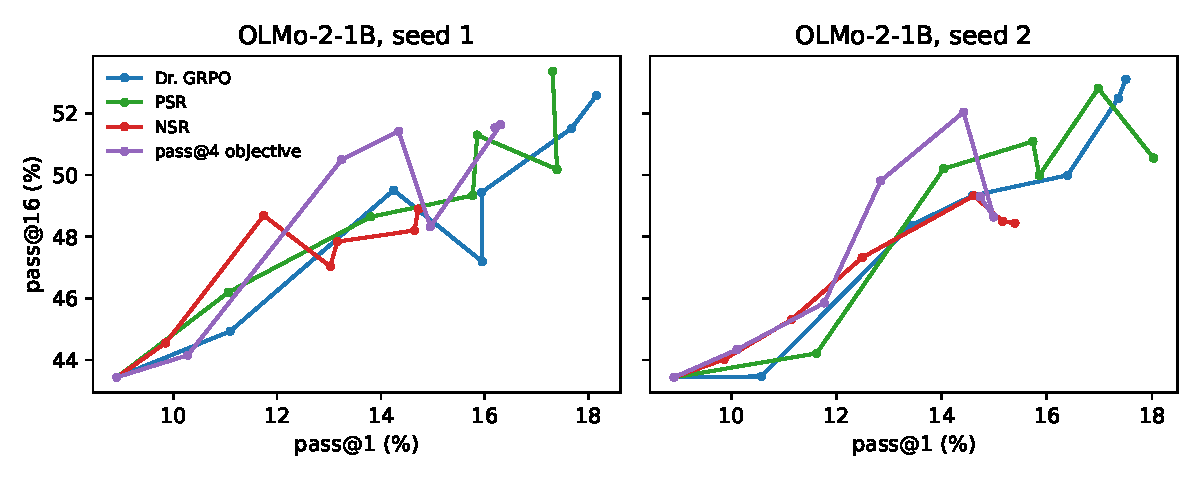
\includegraphics[width=0.85\linewidth]{olmo_curves.pdf}
\caption{OLMo: accuracy (pass@1) against diversity (pass@16) at steps 0 to 300. The rules lie on one curve.}
\end{figure}

\section{Is the noise the cause? (Pre-registration 10)}\label{sec:p10}
\begin{why}
The reviewer's main objection: noise \emph{predicts} learning speed, but in the baseline family more noise always came with a harder push on incorrect answers, so the cause was not shown.
\end{why}
\textbf{The intervention.} Add to PSR a random-sign term whose size, at every step, matches NSR's predicted noise. It averages to zero, so the expected update is unchanged, and it never pushes incorrect answers down systematically. If this ``PSR + noise'' learns as slowly as NSR, noise of that size is enough to cause NSR's lag. Three fresh seeds; also NSR and PSR at twice the learning rate; an NSR ``shadow'' computed on the same answers to check the noise really matches.
\begin{found}
\begin{itemize}[leftmargin=*,itemsep=1pt]
\item The noise matched: 1.02 [1.01, 1.05] times NSR's.
\item \textbf{PSR + noise is as slow as NSR}: speed $\phi=-0.11$ [$-0.22$, $-0.05$] on a scale where NSR is 0 and PSR is 1 (pre-registered margin $\pm1/3$; passed; one seed flagged).
\item NSR at twice the learning rate recovers its whole lag ($\phi=1.16$); at a matched doubled rate the gap shrinks to 31\%.
\item \textbf{Same curve}, now with intervals on Qwen: NSR vs PSR $-0.20$ [$-0.97$, $+0.55$], PSR + noise $-0.37$ [$-1.13$, $+0.46$], NSR at 2$\times$ $-0.03$ (all equivalent within $\pm2$).
\item The noise formula fits training within 0.69--1.18 once gradient sizes are re-measured (the asymmetry fades from about 3$\times$ to 1.5$\times$).
\item Adam: NSR's raw noise is 6$\times$ PSR's but only 1.0--1.3$\times$ after Adam's scaling; NSR's steps point 13--27\% less along the true improvement direction. Noise does not shrink Adam's steps, it misdirects them.
\end{itemize}
\end{found}
\begin{figure}[H]
\centering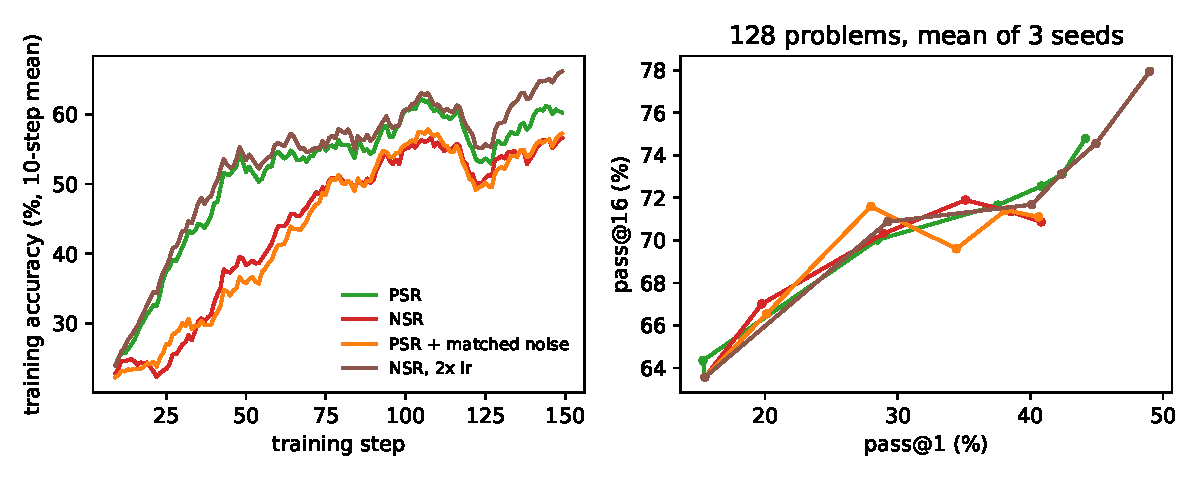
\includegraphics[width=0.85\linewidth]{noise_test.pdf}
\caption{Left: training accuracy; PSR + matched noise (orange) learns as slowly as NSR (red); NSR at twice the learning rate (brown) as fast as PSR (green). Right: all four lie on one accuracy--diversity curve.}
\end{figure}

\section{Is the curve a temperature effect? (Pre-registration 11)}\label{sec:p11}
\begin{why}
By our proposition, diversity at matched accuracy is how evenly success is spread over questions. If RL simply made the model globally more confident (like lowering the temperature), then sampling a late checkpoint at a higher temperature should beat the training curve, and a method that limits sharpening would have room to work. This decides which method to build.
\end{why}
\textbf{Design.} The PSR checkpoints of Pre-registration 10 and the base model, sampled at temperatures 0.5 to 1.6; the quantity $D$ is the late checkpoint's pass@16 at a raised temperature minus the training trajectory's pass@16 at the same pass@1. The model's entropy is also measured on fixed base-model answers.
\begin{found}
\begin{itemize}[leftmargin=*,itemsep=1pt]
\item \textbf{RL does not sharpen globally.} On fixed text the entropy barely changes (1.081 for the base, 1.064 after training), while on the model's own samples it falls three- to fourfold: RL steers into confident paths.
\item \textbf{Undoing sharpening does not help.} At the temperature that restores the base entropy ($T^\ast=1.01$), $D=0.0$ in every seed; slightly higher temperatures stay on the curve; at 1.3 formatting breaks and coverage falls. Pre-registered verdict: inconclusive ($D=-1.54$ on 256 problems; $-1.42$, 90\% [$-2.19$, $-0.68$], on 511).
\item RL is far above anything temperature does for the base model ($+7$ to $+16$ points): RL adds ability, not only sharpening.
\end{itemize}
\textbf{Consequence (declared in advance):} the memory branch of the method experiment runs.
\end{found}
\begin{figure}[H]
\centering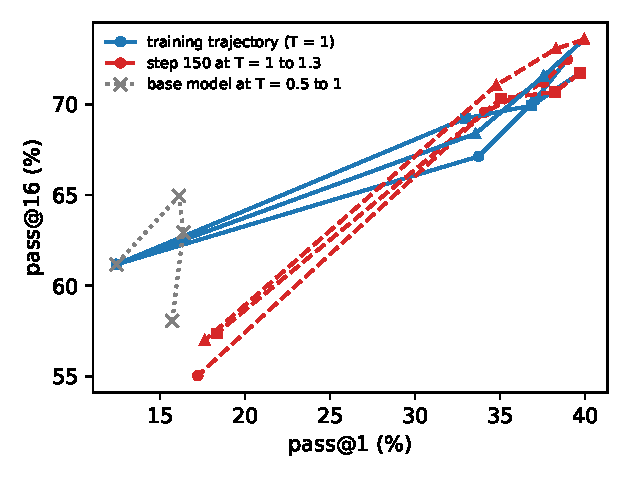
\includegraphics[width=0.5\linewidth]{temperature.pdf}
\caption{Training trajectory (blue), the late checkpoint at higher temperatures (red), and the base model at lower temperatures (gray).}
\end{figure}

\section{Checking the answer keys}
\begin{why}
An independent review found two wrong reference answers in the evaluation sets. Before using them to judge a method, every answer had to be checked.
\end{why}
\begin{found}
Claude Haiku 5.5 solved all 768 evaluation and validation problems; where it disagreed with the key, Claude Opus 5.5 adjudicated. \textbf{3 of 768 keys were wrong (0.4\%)}: a sign error (corrected) and two questions with several answers whose key kept one (excluded). They affect all methods equally; excluding the one in the OLMo set changes no verdict.
\end{found}

\section{From diagnosis to method (Pre-registration 12)}\label{sec:p12}
\subsection{What the diagnosis says a method must do}
\begin{center}\small
\begin{tabularx}{\linewidth}{@{}P{0.46\linewidth}Y@{}}
\toprule
\textbf{Diagnostic finding} & \textbf{Requirement for a method}\\
\midrule
Correctness-only rules (PSR, NSR, baselines, pass@$k$ weights, adaptive sampling) only reweight questions and change noise; they share one curve & Bring in information the current samples do not contain\\
Diversity at matched accuracy = how evenly success is spread across questions & Raise success on rarely solved questions without hurting solved ones\\
On rarely solved questions a group of 8 is usually all wrong, and the signal fades as $p^2(1-p)^2$ & Supply signal exactly there\\
RL does not sharpen globally; entropy control blocks learning & Do not regulate entropy\\
Extra noise slows learning & Keep Dr.\ GRPO's low-noise update as the base\\
\bottomrule
\end{tabularx}
\end{center}

\subsection{The method: coverage-weighted success replay}
\begin{idea}{Coverage-weighted memory (CM)}
Train with Dr.\ GRPO as usual. Store every verified, completed, distinct correct answer the model finds (at most 4 per question). Each step, replay 8 stored questions by adding the gradient of $\lambda\sum_q\log\sum_{y\in S_q}\pi(y\mid q)$, choosing questions in proportion to the expected value of $k\,p(1-p)^{k-1}$ ($k=16$, $p$ the question's estimated success rate). This weight is exactly $\partial\,\mathrm{pass@}k/\partial\log p$: replay goes to questions solved about one time in $k$, whose pass@$k$ can still rise, not to questions already solved.
\end{idea}
Plain replay of stored successes is known (MAPO, self-imitation, STaR, RAFT, ReST); the new parts are the derivation from the diagnosis and the coverage weighting, so uniform replay (M) is run as the ablation at the same strength. Audit arms: the published unlikeliness reward (U), entropy bonus (E), adaptive entropy control (A), and, for the other branch, an entropy floor on the first 32 tokens of each answer (EF).

\subsection{The pilot (one seed, 100 steps, 255 validation problems)}
\begin{center}\small
\resizebox{\linewidth}{!}{\begin{tabular}{@{}lccc@{}}
\toprule
Arm & pass@1 & pass@16 & gain at matched accuracy\\
\midrule
Dr.\ GRPO, steps 0 / 50 / 100 & 15.1 / 35.5 / 39.3 & 63.9 / 71.1 / 72.5 & reference\\
\textbf{Coverage memory, $\lambda=1$ (chosen)} & 35.8 & 73.3 & \textbf{$+2.1$}\\
Coverage memory, $\lambda=4$ & 33.1 & 70.2 & $0.0$\\
Uniform memory, $\lambda=1$ & 38.6 & 72.4 & $+0.2$\\
Uniform memory, $\lambda=4$ & 35.3 & 74.2 & $+3.2$ (4 points slower; excluded by the rule)\\
Entropy bonus & 38.9--39.6 & 72.6--72.7 & about 0\\
Unlikeliness reward & 38.7 & 71.7 & about $-0.5$\\
Adaptive entropy & 9.3--25.5 & 48.9--65.0 & $-2.5$ or collapsed\\
Early-token entropy floor & 12.6--12.8 & 56.1--58.6 & collapsed (below the base model)\\
\bottomrule
\end{tabular}}
\end{center}
\textbf{Reading.} Memory is the only family that lifts the curve; at the same strength, coverage weighting gives $+2.1$ against $+0.2$ for uniform replay (one seed, noise about $\pm2$). Entropy-based fixes do not help or break learning, as the diagnosis predicted.

\subsection{The main runs: results}
Seeds 8, 9, 10; Dr.\ GRPO (B), coverage memory (CM, $\lambda=1$), uniform memory (M) and the unlikeliness reward (U), 150 steps; evaluation on 511 held-out problems with 32 samples at steps 50, 100, 150, B also at $T=1.15$ and $1.3$; greedy accuracy on 3,382 test problems. Rule: CM \emph{moves the curve} if at least $+2$ points above B's trajectory-and-temperature envelope with the 95\% interval above 0 in every seed.

\begin{center}\small
\resizebox{\linewidth}{!}{\begin{tabular}{@{}lcccc@{}}
\toprule
Arm & Gain at matched pass@1 & 95\% interval & Step-150 pass@1 / pass@16 & Greedy test accuracy\\
\midrule
Dr.\ GRPO (B) & 0 & & 44.1 / 74.5 & 47.9\\
Coverage memory (CM) & $+1.19$ (per seed $+1.52$, $+1.44$, $+0.59$) & $[+0.54,+1.79]$ & 42.1 / 75.2 & 47.7\\
Uniform memory (M) & $+0.61$ & $[-0.04,+1.27]$ & 42.9 / 74.0 & 47.3\\
Unlikeliness (U) & $+0.14$ & $[-0.32,+0.62]$ & 43.4 / 74.0 & 47.6\\
\bottomrule
\end{tabular}}
\end{center}
\begin{found}
Registered verdict for CM: \textbf{average agreement} (90\% interval $[+0.63,+1.69]$ inside $\pm2$). A small, consistent lift, larger than uniform replay and the published unlikeliness reward, but half the registered bar. Coverage weighting over uniform replay ($+0.66$) misses its $+1$ bar; CM's step-150 pass@1 is 2.05 points below B's; greedy accuracy differs by $-0.18$, 90\% $[-0.83,+0.43]$. Both memory arms used the archive on 100\% of steps after step 20. Interpretation: a group of 8 finds a success on a problem with $p=1/16$ only 40\% of the time ($p=1/32$: 22\%), so the policy's own archive misses most of the problems whose pass@16 can still rise.
\end{found}

%=====================================================================
\section{The 2026 literature, and what it changed}\label{sec:lit2026}
\begin{why}
Before choosing the next method, we searched arXiv (October 21) for 2025--2026 work on the diagnosis and on methods (two systematic searches, every abstract opened, the closest papers read in full).
\end{why}
\begin{found}
\begin{itemize}[leftmargin=*,itemsep=1pt]
\item \textbf{Theory, partly prior:} binary-reward RL as ascent on transforms of per-problem success (Davis and Recht, 2510.13651), weight-dependent convergence (Heckel et al., 2602.11128), pass@$k$ advantage shaping as surrogate rewards (Thrampoulidis et al., 2510.23049), pass@$k$ gradients as reweighted pass@1 gradients (2511.16231). Barakat et al.\ (2602.21189, NeurIPS 2026) show that reweighting toward hard prompts can rotate the aggregate update through shared parameters, so ``one curve'' must be an empirical claim.
\item \textbf{Methods, largely covered in pieces:} base-seeded replay with a likelihood gate (TAR, 2610.24236); base-model archives for replay (EliteReplay, 2610.22290); a Bayesian pass@16 gate close to our coverage weight (BBG, 2606.15455); off-policy rescue of zero-success groups (LSPO, 2607.27787; LUFFY, 2504.14945; ExGRPO, 2510.02245); rollout allocation by posterior hit utility with per-problem normalization (HORA, 2605.07114); Knapsack RL (2509.25849); DARS (2508.13755), which adds rollouts for low-accuracy problems and plots Pass@1--Pass@$K$ curves; MaxRL (2602.02710, ICML 2026); transfer-driven curricula (TAC, 2606.25178; GradAlign, 2602.21492).
\item \textbf{Not found:} the noise-injection test; matched-pass@1 evaluation of advantage rules with intervals and registered rules on two families; the temperature control. DARS compares Pass@1--Pass@$K$ curves informally (no intervals or protocol).
\end{itemize}
Codex's re-assessment after the search: about 5/10 for the diagnosis alone; the method side needs to beat the closest published methods, not only Dr.\ GRPO.
\end{found}

%=====================================================================
\section{Seeding the memory from the base model (Pre-registration 14)}\label{sec:p14}
\begin{why}
Pre-registration 12 showed the bottleneck is discovery: the policy rarely finds a success on a rarely solved problem. Thirty-two base-model samples per problem raise the chance of finding one to 87\% at $p=1/16$ and 64\% at $p=1/32$. Seeding the archive with these discoveries tests whether replay can reach the tail.
\end{why}
\textbf{Discovery.} The base model sampled 32 answers for each of the 3,920 training problems (125,440 completions): 3,433 problems solved at least once; 3,235 with a retained success (correct, stop-terminated, parseable final box), including 988 of the 1,181 problems with 1--4 successes.

\textbf{Arms} (seeds 8--10, Pre-registration 12's settings): D32, seeded coverage-weighted memory at $\lambda=0.5$ (candidate); U32, seeded uniform memory; S32, a supervised warm start on the same successes (AdamW $10^{-5}$, 2.46 million response tokens) followed by Dr.\ GRPO; C05, unseeded coverage memory at $\lambda=0.5$; G32, Dr.\ GRPO with groups of 32 (amendment 2); T32, TAR's gated replay on the same archive (amendment 4). Holm's correction over seven tests; a joint win needed $\ge+2$ points and step-150 pass@1 within $\pm1$ of B.

\begin{found}
\begin{itemize}[leftmargin=*,itemsep=1pt]
\item D32 against B's envelope: $+1.02$, 95\% $[+0.23,+1.68]$, per seed $+0.71$, $+1.23$, $+1.12$: average agreement; step-150 pass@1 5.35 points below B. No joint win.
\item D32 against U32's trajectory $-0.39$ (coverage weighting does not help); against C05's $+0.92$ (seeding adds less than $+1$); against S32's: insufficient overlap. U32 against B (reported): $+1.37$; C05: $+0.33$.
\item S32 and G32 leave B's accuracy range: both end at step-150 pass@1 52.5 (B: 44.1), pass@16 78.7 and 78.9. S32's pass@16 increase over B is concentrated on problems the base never solved in 32 samples (24.0 $\to$ 34.2, \cref{fig:strata}).
\item In training, S32 starts at 54--59\% accuracy right after the supervised stage and ends near 71\% (B: 60--63\%); D32 learns the training problems more slowly (56--58\%). About 1,500 of the 3,220 seeded traces were still unretired at step 150. T32's evaluation is pending.
\end{itemize}
\end{found}

\begin{figure}[H]
\centering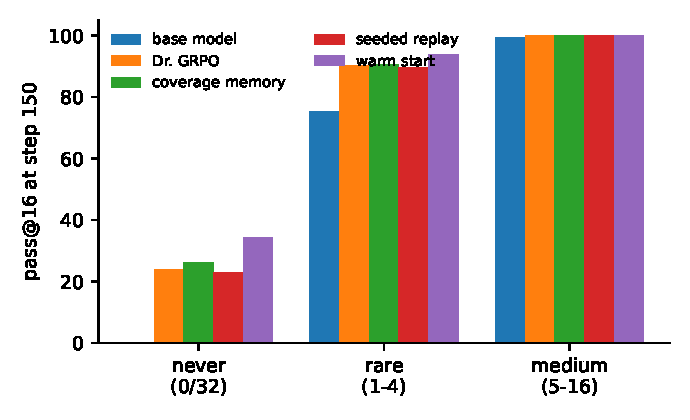
\includegraphics[width=0.62\linewidth]{strata.pdf}
\caption{pass@16 at step 150 by the base model's successes in 32 samples on each test problem.}
\label{fig:strata}
\end{figure}

%=====================================================================
\section{Checking the answer budget (Check 16)}
\begin{why}
At 512 tokens, 48\% of Dr.\ GRPO's sampled answers at step 150 are truncated (S32: 33\%; D32: 59\%). If hard problems need longer answers, part of S32's gain could be ``finishes within the budget''.
\end{why}
\begin{found}
Re-evaluated at 1,024 tokens (partial): the base model reaches pass@1 21.6 and pass@16 79.3 (36.2\% truncated; 14.1 and 62.6 at 512); Dr.\ GRPO seed 10 at step 150 reaches 57.7 and 88.4 (15.5\% truncated; 44.6 and 75.2 at 512); S32 seed 9 reaches 63.8 and 89.7 (4.9\%). Absolute values depend strongly on the budget; the warm start's pass@1 advantage shrinks from about 8.7 to about 6.1 points (different seeds). Every comparison in this document is within one budget.
\end{found}

%=====================================================================
\section{2026 methods at matched accuracy (Pre-registration 15)}
\begin{why}
If the diagnosis is right, recent methods that report pass@$k$ gains at fixed steps should also lie on the curve at matched pass@1. The audit also supplies the baselines a method must beat.
\end{why}
\textbf{Arms} (seeds 8--10, our recipe): BBG (W-REINFORCE with positive weight 0.3, gated by the posterior mean of $16(1-p)^{15}$, coefficients rescaled to mean 1 per step), W-REINFORCE (BBG's base, positive weight 0.3), MaxRL (advantages $(r-\bar r)/\bar r$, none for zero-success groups); TAR is part of Pre-registration 14. Holm over the three directional tests.
\begin{found}
Interim (training complete for most seeds, evaluation partial): BBG progresses much more slowly than Dr.\ GRPO (seed 9: pass@1 18.4, 24.8, 29.8 at steps 50, 100, 150). Its apparent gains ($+1.3$ to $+2.6$) lie between the base model and Dr.\ GRPO's step 50, where the registered reference is a straight chord that understates a concave trajectory. Check 20 adds Dr.\ GRPO checkpoints at steps 10--40 to measure that bias.
\end{found}

%=====================================================================
\section{Pushing signal onto rare problems inside RL (Pre-registration 16, pilot)}
\begin{why}
The PI asked for a method inside RL rather than a supervised stage. Replay delivered far less push than the warm start, so this pilot tests stronger mechanisms on rarely solved problems.
\end{why}
\textbf{Candidates} (seed 12, 255 validation problems): AR, annealed replay (seeded coverage replay at $\lambda=4$ falling to 0 by step 100, 16 problems replayed per step); GC, group completion (a stored success appended to a zero-success group as a ninth answer); PG, prefix-guided rollouts (for problems with at most 4 base successes in 32, two of eight rollouts continue from the first $f_t$ of a stored success, $f_t=0.5(1-t/100)$); MXGC, MaxRL with group completion. References: B, S32, SD (S32 plus seeded replay), MXR. Selection: the largest gain $\ge+1.5$ with step-150 pass@1 within 2 points of B.
\begin{found}
Interim: AR $+1.30$ and MXGC $+1.12$ at matched pass@1, but with step-150 pass@1 6.6 and 6.5 points below B, so neither qualifies. S32 is 8.5 points above B in pass@1 (beyond B's range). GC and PG are being evaluated; SD and MXR are training.
\end{found}

%=====================================================================
\section{Does training transfer to rarely solved problems? (Check 17)}
\begin{why}
An idea discussed with the PI: a problem the policy never solves contributes nothing itself and can only improve through the effect of updates on other problems. If Dr.\ GRPO transferred little to rare problems while the warm start transferred much, a transfer-targeted method would follow. (Codex found that transfer-driven curricula, TAC and GradAlign, already exist, so the method version was dropped; the measurement was kept.)
\end{why}
\textbf{Probe.} For 395 held-out problems (149 with 1--4 base successes, 246 with 5--16), up to four correct and four incorrect base answers with a parseable final box. For each checkpoint, $\ell(y)=|y|^{-1}\log\pi(y\mid x)$; per problem the margin $m_x=\bar\ell_{\rm correct}-\bar\ell_{\rm incorrect}$; transfer $=\Delta m_x$ relative to the base model.
\begin{found}
Four of six lanes: Dr.\ GRPO's margin rises by $+0.025$ on both rare and medium problems by step 150 (seed 8), and $+0.023$ and $+0.024$ (seed 10). S32: $+0.049$ and $+0.063$ (seed 9), $+0.058$ and $+0.070$ (seed 10), of which most comes from the supervised stage. The premise that Dr.\ GRPO transfers little to rare problems is \textbf{not supported}.
\end{found}

%=====================================================================
\section{A model of the frontier (Pre-registration 17)}\label{sec:p17}
\begin{why}
Looking across all per-problem counts, one regularity stood out: the observed frontier looks like what one gets if each problem's log-odds grow only with its own signal. If a frozen model of that kind predicts new methods, model families and budgets, the frontier is a property of the base model's difficulty distribution, and the reward rule only sets the progress.
\end{why}
\begin{idea}{Model}
$\theta_x(0)=\log\frac{c_x+a}{n-c_x+b}$ from the base model's counts (Beta$(a,b)$ by moments), $\dot\theta_x=p_x(1-p_x)+\tau\,\overline{p(1-p)}$. A checkpoint is placed where the model's mean success equals its pass@1; the model then predicts pass@$k$ for $k>1$, strata and per-problem counts. $\tau=-0.20$ fitted once on Dr.\ GRPO's nine checkpoints, then frozen (code committed before any test).
\end{idea}

\begin{center}\small
\resizebox{\linewidth}{!}{\begin{tabular}{@{}lccc@{}}
\toprule
Test set & checkpoints & pass@16 RMSE: model / uniform shift / affine & criterion ($\le2$)\\
\midrule
Nine other rules, Qwen & 56 & \textbf{1.21} / 20.07 / 2.45 & met\\
OLMo, five rules, $\tau$ from Qwen & 50 & \textbf{1.90} / 9.85 / 12.58 & met\\
1,024 tokens & 4 & \textbf{0.85} / 11.48 / 1.27 & met\\
Warm start, from its own step-0 counts & 9 & 3.56 / 9.04 / 7.99 & not met\\
\bottomrule
\end{tabular}}
\end{center}

\begin{figure}[H]
\centering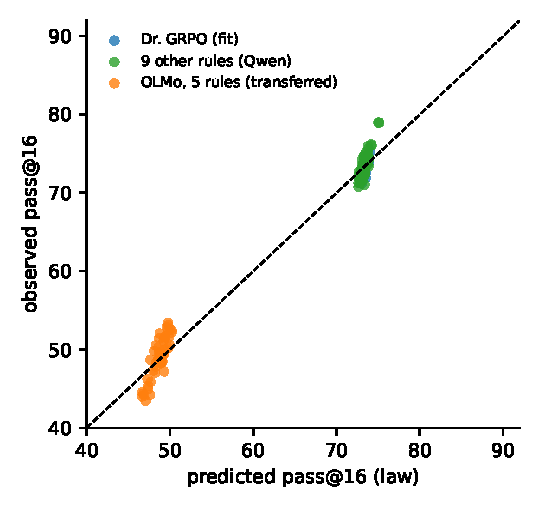
\includegraphics[width=0.45\linewidth]{law_fit.pdf}
\caption{Predicted against observed pass@16 for the frozen model.}
\end{figure}

\begin{found}
\begin{itemize}[leftmargin=*,itemsep=1pt]
\item Within the trained range the model reproduces the frontier of rules it never saw, of a second family and of a second budget; a uniform log-odds shift would put never-solved problems at 70--80 pass@16, the data at 24. Diversity collapse is a state-dependent concentration of success.
\item After the warm start it fails ($c=0$ stratum $-11.92$ points; refitted $\tau=-0.65$ to $-0.70$): the supervised stage changes the subsequent dynamics.
\item Deep base sampling (256 more samples on 232 of the 309 problems with $c\le4$): 53\% of the never-solved problems are solved at least once, at a mean rate of 0.93\%; with these counts $\tau=+0.20$, 90\% $[+0.10,+0.35]$: weak positive transfer.
\item \textbf{Extrapolation fails}: on the 450-step run the frozen model is 2.0 and 3.6 points too low at steps 200 and 250 (1.6 and 2.7 with the deep counts). It describes the frontier within the trained range; it is not a law that extrapolates.
\end{itemize}
\end{found}

%=====================================================================
\section{Faster, not better: the long Dr.\ GRPO run}\label{sec:long}
\begin{why}
S32 and G32 leave Dr.\ GRPO's 150-step range, so the registered comparison is undefined for them. A Dr.\ GRPO run to 450 steps (seed 13) supplies the missing reference.
\end{why}
\begin{found}
Dr.\ GRPO seed 13 reaches (pass@1, pass@16) = (36.6, 72.0), (40.3, 71.1), (43.5, 74.1), (48.3, 76.5), (51.7, 78.6) at steps 50--250. Against this single trajectory at matched pass@1: Dr.\ GRPO's seeds 8--10 $+0.47$ (the reference seed's own noise), \textbf{G32 $+0.60$}, \textbf{S32 $+2.38$}, CM $+1.73$, U32 $+1.74$, D32 $+1.06$, C05 $+0.82$. Four times as many rollouts buy speed, not a better trade-off; Dr.\ GRPO reaches the same point with fewer rollouts (32,000 against 76,800). The warm start is the only clear departure, about two points above. Steps 300--450 and seeds 14--15 are pending.
\end{found}

\begin{figure}[H]
\centering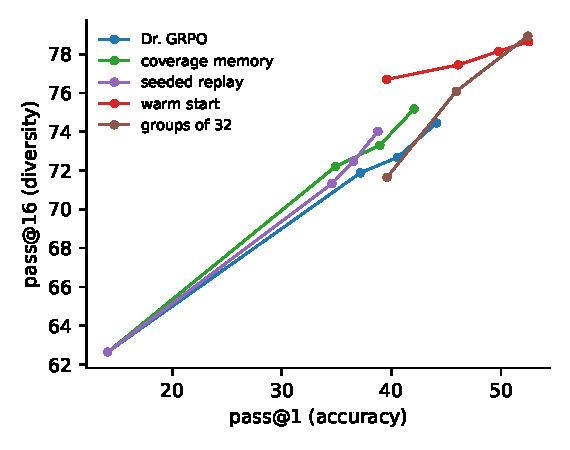
\includegraphics[width=0.6\linewidth]{frontier_qwen.pdf}
\caption{Seed-mean trajectories on Qwen, with the long Dr.\ GRPO run (dashed).}
\end{figure}

%=====================================================================
\section{Allocating rollouts by frontier value (Pre-registration 18, running)}
\begin{why}
By \cref{lem:starve-story} below, a rarely solved problem moves only when a group contains a success, which happens with probability about $np$; the number of rollouts it receives is the one lever that reweighting cannot replace. The frozen model makes a quantitative forecast for three ways of spending the same rollout budget.
\end{why}
\textbf{Arms} (seeds 8--10; exactly 128 rollouts per step as B: 4 per problem, then 64 extras, at most 32 per problem). AC: extras in proportion to the frontier value under the model, $\max\{0,\E[p^2(1-p)^2(16(1-p)^{15}-\lambda)]\}$, $\lambda=0.37$ (B's observed frontier slope); only problems with no pilot success have positive value. AV: extras in proportion to $\E[p(1-p)]$ (signal per rollout). HR: HORA's greedy hit utility with per-problem normalization. Forecasts (gain over B at matched pass@1, frozen model / deep-count variant): AC $+4.34$ / $+2.56$; HR $+0.15$ / $+0.07$; AV $-1.13$ / $-0.72$. Rules: AC $\ge+2$ against B; AC against AV and against HR each $\ge+1$; Holm over three. Status: AC and AV training on AWS; HR on Vulcan.

\section{External versus self-generated information (Pre-registration 19, running)}
\begin{why}
If interventions that reuse the policy's own information only add speed, information the base model does not have should move the frontier.
\end{why}
\textbf{Data}: human-written MATH solutions for all 3,920 training problems (all verified). \textbf{Arms} (supervised stage as S32, then Dr.\ GRPO): HQ, 3,433 problems in which 487 randomly chosen problems with $c>0$ are replaced by the 487 never-solved problems; HP, the 3,433 problems with $c>0$; HS, the 3,235 problems of S32. Rule: HQ against HP's trajectory $\ge+1$ with the 95\% interval above 0 (same size and token budget; they differ only in whether 487 slots hold never-solved problems). Stated confounds: the never-solved problems' solutions are about twice as long (fewer epochs at the fixed token budget, about 12\%); ``never solved in 32 samples'' is not ``unsolvable''. Status: one run training on AWS, eight queued on Vulcan.

\section{Early reference checkpoints (Check 20, running)}
Dr.\ GRPO for 50 steps, seeds 8--10, checkpoints at 10, 20, 30, 40, 50, evaluated on the 511 problems (Nibi H100s), to replace the base-to-step-50 chord for slow arms; reported as a sensitivity analysis.

\begin{lemma}[stated for reference]\label{lem:starve-story}
Under Dr.\ GRPO with a group of $n$, the update on a problem is zero unless the group contains both a correct and an incorrect answer, probability $1-p^n-(1-p)^n\approx np$ for small $p$; reweighting by a function of the rewards does not change this.
\end{lemma}

%=====================================================================
\section{Where we stand, and the path to ICML}
\subsection{What is established}
\begin{enumerate}[leftmargin=*,itemsep=1pt]
\item Per problem, every correctness-only advantage rule has expected update $c(p_x)\nabla p_x$; the second moment follows from four quantities; incorrect answers carry 2--3 times larger squared score norms.
\item At matched pass@1, NSR, PSR, constant baselines, the NSR paper's implementation, a pass@4 objective and the unlikeliness reward lie within about $\pm2$ points of one trajectory on two families; trace-matched noise reproduces NSR's lag; a hotter late checkpoint does not exceed the trajectory.
\item Interventions that add the policy's or the base model's own samples (replay, seeded replay, groups of 32) change the progress rate and move the frontier by at most about one point; the supervised warm start on base successes is the only clear departure (about two points, one reference seed).
\item A frozen per-problem model predicts the frontier within the trained range across rules, families and budgets, but not after a warm start and not far beyond the trained range.
\end{enumerate}

\subsection{Open questions}
\begin{itemize}[leftmargin=*,itemsep=1pt]
\item Does allocation by frontier value move the frontier at an equal rollout budget, and beat HORA (Pre-registration 18)?
\item Does external information move it where self-generated information does not (Pre-registration 19)?
\item The long-run reference with three seeds; the 2026 methods with the early-checkpoint reference; TAR.
\item Scale: Qwen2.5-Math-7B at 2,048 tokens (multi-GPU training on Nibi or Fir).
\end{itemize}

\subsection{Independent review over time}
\begin{center}\small
\begin{tabular}{@{}ll@{}}
\toprule
Stage & Score (Codex)\\
\midrule
Qwen experiments only & 4/10\\
+ noise-injection test & 5/10\\
+ OLMo replication & 6/10\\
After the 2026 literature search & about 5/10\\
Scenario: the frontier model passes its remaining tests & about 7/10\\
Scenario: a method that improves the frontier across scales & about 8/10\\
\bottomrule
\end{tabular}
\end{center}

\subsection{Three months to ICML}
\begin{itemize}[leftmargin=*,itemsep=1pt]
\item \textbf{November:} verdicts of Pre-registrations 18 and 19; long-run reference with three seeds; multi-GPU training code; 7B core runs (Dr.\ GRPO, PSR/NSR, the best method) at 2,048 tokens on Nibi or Fir.
\item \textbf{December:} 7B results; OLMo replication of the method or thesis; full matched-pass@1 audit of 2026 methods.
\item \textbf{January:} writing (draft v1 in \texttt{paper/icml/}), internal review with Codex, submission.
\end{itemize}

\appendix
\section{Methods reference}\label{app:methods}
\small
\begin{longtable}{@{}P{3.0cm}P{6.2cm}P{4.6cm}@{}}
\toprule
\textbf{Rule} & \textbf{Definition} & \textbf{Settings}\\
\midrule
\endhead
Dr.\ GRPO (B) & $A_i=r_i-\bar r$ within a group of $n$; loss $-(PnL)^{-1}\sum_iA_i\sum_t\log\pi(y_{it})$ & $P=16$, $n=8$, $L=512$, AdamW $10^{-6}$, 150 steps, on-policy\\
PSR / NSR & $A=r$ / $A=r-1$ & as B\\
W-REINFORCE & $A=w$ if correct, $-1$ if incorrect & $w=0.1$ (Zhu et al.) or $0.3$ (BBG)\\
Constant baselines & $A=r-b$ & $b\in\{0,0.25,0.5,0.75,1\}$\\
pass@$k$ objective & unbiased pass@4 weights with leave-one-out baseline & $k=4$, $n=8$\\
PSR + noise & $A_i=r_i+c_ts_i$, $s_i=\pm1$ & $c_t^2$ matches NSR's predicted second moment\\
Unlikeliness reward & correct samples in mixed groups get $1-\beta(G-\mathrm{rank})/G$ & $\beta=0.25$\\
Coverage memory (CM) & add $\lambda\nabla\sum_q\log\sum_{y\in S_q}\pi(y\mid q)$ over 8 archived problems sampled $\propto\E[k\,p(1-p)^{k-1}]$, $p\sim\mathrm{Beta}(c+\frac12,n-c+\frac12)$ & $\lambda=1$, $k=16$, $\le4$ successes per problem\\
Uniform memory (M) & as CM with uniform sampling & $\lambda=1$\\
Seeded memory (D32, U32) & archive initialized with one base success per problem; retired at the first own success & $\lambda=0.5$\\
Warm start (S32) & mean token NLL on base successes, then B & AdamW $10^{-5}$, batches of 8, 2.46M tokens, clip 1, optimizer reset\\
Groups of 32 (G32) & B with $n=32$ & 512 rollouts per step\\
TAR & $\lambda\,\mathrm{mean}_{\tau}\,\mathrm{sg}[g]\sum_t\mathrm{sg}[w_t](-\log\pi_t)/(\epsilon+\sum_t\mathrm{sg}[w_t])$, $g=\phi(\overline{\delta})$, $w_t=\phi(\delta_t)$, $\delta_t=\log\pi_{\rm base}-\log\pi$ & $\lambda=1$, 16 replayed per step\\
BBG & W-REINFORCE times $\alpha(m)=u(m;8,16)\mathbf 1[u\ge0.09]$, $u=16\prod_{j=1}^{15}\frac{8-m+j}{9+j}$, rescaled to mean 1 & $w=0.3$\\
MaxRL & $A=(r-\bar r)/\bar r$; 0 if $\bar r=0$ & as B\\
Annealed replay (AR) & seeded coverage replay, $\lambda_t=4(1-t/100)_+$ & 16 problems per step\\
Group completion (GC) & stored success appended to zero-success groups ($n+1$ answers, Dr.\ GRPO advantages) & no importance weight\\
Prefix-guided (PG) & 2 of 8 rollouts continue from $f_t$ of a stored success; prefix is context & $f_t=0.5(1-t/100)_+$, problems with $c\le4$ of 32\\
Allocation (AC, AV, HR) & 4 pilot rollouts per problem, 64 extras by value (frontier value, signal, or HORA hit utility) & 128 rollouts per step, $\le32$ per problem\\
\bottomrule
\end{longtable}
\normalsize
\textbf{Evaluation.} 511 held-out MATH test problems (labels audited), 32 samples at $T=1$, unbiased pass@$k$; greedy accuracy on 3,382 problems; matched-pass@1 interpolation along B's trajectory and temperature envelope; 2,000 bootstrap draws over problems; Holm's correction within each registration.

\section{Experiment tracker (Pre-registrations 13--20)}
\small
\begin{longtable}{@{}P{0.9cm}P{3.3cm}P{4.6cm}P{5.2cm}@{}}
\toprule
\textbf{\#} & \textbf{Question} & \textbf{Design} & \textbf{Result}\\
\midrule
\endhead
12 & Does coverage memory move the curve? & 4 arms, 3 seeds, 511 problems & $+1.19$ $[+0.54,+1.79]$: average agreement\\
13 & OLMo replication of the method & planned & not run (the method did not pass)\\
14 & Base-seeded memory and controls & D32, U32, S32, C05, G32, T32; 3 seeds & D32 $+1.02$, slower; S32 and G32 beyond B's range; T32 pending\\
15 & 2026 methods at matched pass@1 & BBG, W-REINFORCE, MaxRL; 3 seeds & interim: BBG slow, apparent gains in the chord region\\
16 & Push mechanisms inside RL (pilot) & AR, GC, PG, MXGC + refs; 1 seed & interim: AR, MXGC not eligible; GC, PG pending\\
C16 & 512 vs 1,024 tokens & re-evaluation & partial: all values rise at 1,024\\
C17 & Transfer to rare problems & likelihood margins of fixed base answers & 4/6 lanes: Dr.\ GRPO transfers to rare as to medium\\
17 & Frontier model & frozen model, 5 test sets & met on 3, not met after warm start; extrapolation too low\\
18 & Allocation by frontier value & AC, AV, HR; 3 seeds; registered forecasts & running\\
19 & External vs self-generated information & HQ, HP, HS; 3 seeds & running\\
C20 & Early reference checkpoints & B steps 10--50, 3 seeds & running\\
\bottomrule
\end{longtable}
\normalsize

\section{Compute and engineering}
Training and evaluation ran on AWS SageMaker (L40S GPUs, g6e instances; launched in three regions, keeping the first copy to start), and from October 22 also on Alliance clusters: Tamia (H100; low scheduling priority), Vulcan (L40S, the same GPU as AWS) and Nibi (H100). Engineering issues fixed in this period: spot jobs expiring after 22 hours without capacity (relaunched on demand); a PyTorch 2.14 build producing non-finite gradients on H100 (environment rebuilt with 2.9.1; updates with non-finite gradient norms are now skipped and logged); SLURM jobs killed for host memory (whole-node memory requested). All code, registrations, results and figures: \texttt{github.com/mayman150/rlvr-adaptive}.

\end{document}
